\documentclass[tikz]{standalone}
\usetikzlibrary{calc}
\usepackage{pgfplots}
\usepgfplotslibrary{polar}
\pgfplotsset{compat=1.13}

\begin{document}

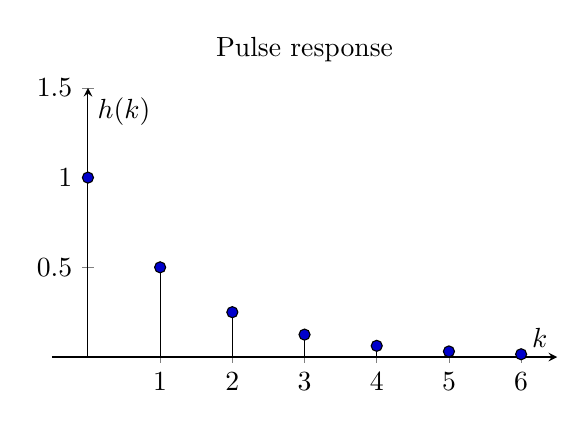
\begin{tikzpicture}
\begin{axis}[
  width=8cm,
  height=5cm,
  xlabel={$k$},
  ylabel={$h(k)$},
  axis lines=middle,
  xmin=-.5,
  xmax=6.5,
  ymin = 0, ymax = 1.5,
  xtick = {1,2,3,4,5,6},
  title={Pulse response},
]

\addplot+[black, ycomb, domain=-2:10, samples=13,variable=k] { (k>-1)*pow(0.5,k)}; 

\end{axis}
\end{tikzpicture}
\end{document}
